\documentclass[tikz,border=4pt]{standalone}
\usepackage{fontspec,amsmath,amssymb,unicode-math}
\setmainfont{STIXTwoText-Regular.otf}[BoldFont=STIXTwoText-Bold.otf,ItalicFont=STIXTwoText-Italic.otf]
\setmathfont{STIXTwoMath-Regular.otf}
\usetikzlibrary{arrows.meta,positioning,calc}
\definecolor{hmtgold}{RGB}{145,101,26}
\definecolor{hmtviolet}{RGB}{92,64,125}
\definecolor{hmtgray}{RGB}{87,95,102}
\definecolor{hmtpaper}{RGB}{248,247,243}
\definecolor{hmtlightgold}{RGB}{249,242,225}
\definecolor{hmtlightviolet}{RGB}{241,236,248}
\begin{document}
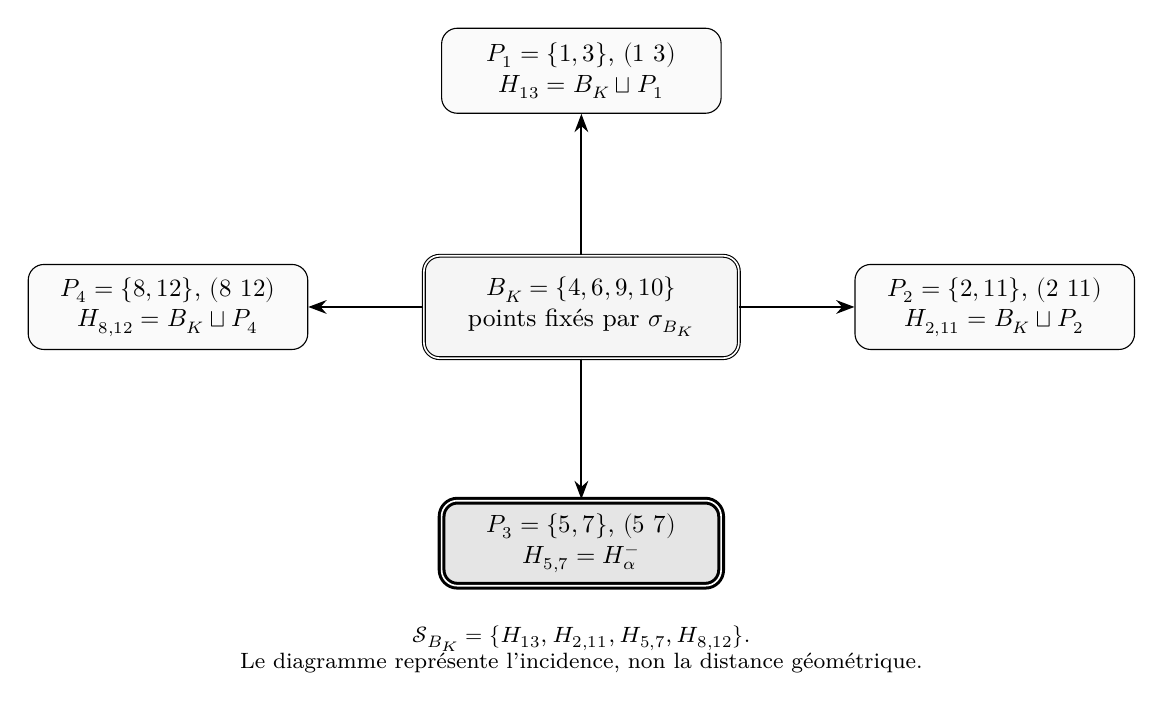
\begin{tikzpicture}[
  >=Stealth,
  font=\small,
  core/.style={draw,double,rounded corners=2mm,align=center,
    minimum width=4.0cm,minimum height=1.3cm,fill=black!4},
  petal/.style={draw,rounded corners=2mm,align=center,
    minimum width=3.55cm,minimum height=1.08cm,fill=black!2},
  negative/.style={petal,line width=1.1pt,double,fill=black!10},
  arr/.style={->,thick}
]
\node[core] (B) at (0,0)
 {\(\displaystyle B_K=\{4,6,9,10\}\)\\
  points fixés par \(\sigma_{B_K}\)};
\node[petal] (P13) at (0,3.0)
 {\(P_1=\{1,3\}\), \((1\ 3)\)\\
  \(H_{13}=B_K\sqcup P_1\)};
\node[petal] (P211) at (5.25,0)
 {\(P_2=\{2,11\}\), \((2\ 11)\)\\
  \(H_{2,11}=B_K\sqcup P_2\)};
\node[negative] (P57) at (0,-3.0)
 {\(P_3=\{5,7\}\), \((5\ 7)\)\\
  \(H_{5,7}=H_\alpha^-\)};
\node[petal] (P812) at (-5.25,0)
 {\(P_4=\{8,12\}\), \((8\ 12)\)\\
  \(H_{8,12}=B_K\sqcup P_4\)};
\draw[arr] (B)--(P13);
\draw[arr] (B)--(P211);
\draw[arr] (B)--(P57);
\draw[arr] (B)--(P812);
\node[align=center,font=\footnotesize] at (0,-4.35)
 {\(\mathscr S_{B_K}
   =\{H_{13},H_{2,11},H_{5,7},H_{8,12}\}\).\\
  Le diagramme représente l’incidence, non la distance géométrique.};
\end{tikzpicture}
\end{document}
